% 2011 年四川卷文科第 15 题：半径为 4 的球 O 及其内接圆柱。
% 来源 PDF：普通高考/2011/2011四川文.pdf，SHA-256 9df4a6b69bb06bfab2f7d7ee0e7fcc50ae547f226260996d7a060c31ad14e64a。
% 原页：第 1 页（A3 三栏）第 2 栏下部，书页码 703。
% 重绘依据：照原页——外轮廓为球的大圆；圆柱上下底画成扁椭圆，上底后半弧虚线、前半弧实线，
%   下底后半弧虚线、前半弧实线；圆柱两条母线为虚线；O 为球心（实心点，标注在点的左侧）。
%   原页不画赤道、不标半径，照录。上底圆周左右两端恰落在球的大圆上，母线在球内。
%   取 r=0.8R、高=1.2R（即 r^2+(h/2)^2=R^2，球与圆柱确为内接关系），椭圆短半轴取 0.34，不严格按比例。
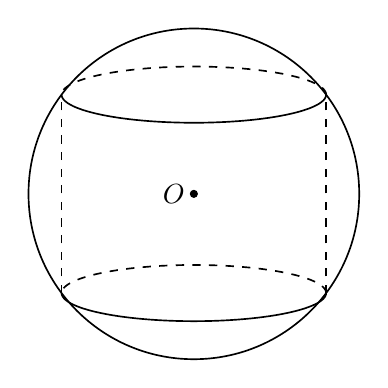
\begin{tikzpicture}[scale=1.05, >=stealth, semithick]
  % 球的大圆
  \draw (0,0) circle (2);

  % 圆柱上底：后半（上）虚线，前半（下）实线
  \draw[domain=0:180, samples=60, dashed] plot ({1.6*cos(\x)},{1.2+0.34*sin(\x)});
  \draw[domain=180:360, samples=60] plot ({1.6*cos(\x)},{1.2+0.34*sin(\x)});

  % 圆柱下底：后半（上）虚线，前半（下）实线
  \draw[domain=0:180, samples=60, dashed] plot ({1.6*cos(\x)},{-1.2+0.34*sin(\x)});
  \draw[domain=180:360, samples=60] plot ({1.6*cos(\x)},{-1.2+0.34*sin(\x)});

  % 圆柱的两条母线（原页为虚线）
  \draw[dashed] (-1.6,-1.2) -- (-1.6,1.2);
  \draw[dashed] (1.6,-1.2) -- (1.6,1.2);

  % 球心
  \fill (0,0) circle (1.4pt);
  \node[left, inner sep=3pt] at (0,0) {$O$};
\end{tikzpicture}
